

\tikzset{every picture/.style={line width=0.75pt}} %set default line width to 0.75pt        

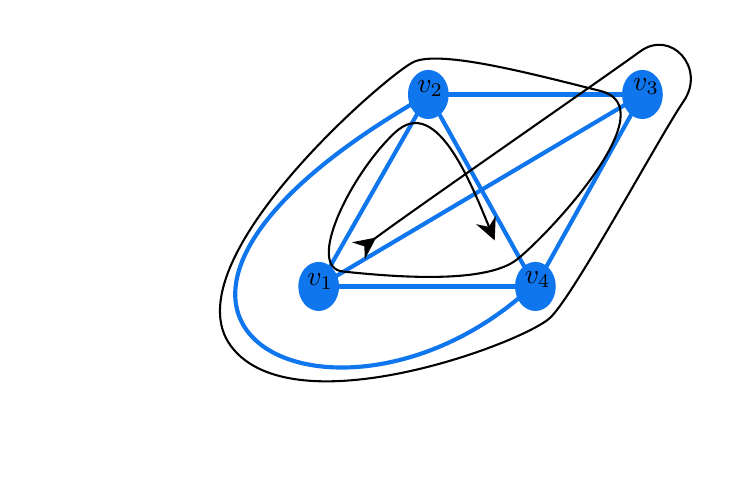
\begin{tikzpicture}[x=0.75pt,y=0.75pt,yscale=-1,xscale=1]
%uncomment if require: \path (0,191); %set diagram left start at 0, and has height of 191

%Shape: Ellipse [id:dp14942589100099868] 
\draw  [draw opacity=0][fill={rgb, 255:red, 15; green, 118; blue, 237 }  ,fill opacity=1 ] (241.97,36.83) .. controls (241.97,30.3) and (246.37,25) .. (251.79,25) .. controls (257.22,25) and (261.61,30.3) .. (261.61,36.83) .. controls (261.61,43.37) and (257.22,48.67) .. (251.79,48.67) .. controls (246.37,48.67) and (241.97,43.37) .. (241.97,36.83) -- cycle ;
%Shape: Ellipse [id:dp26449670264630165] 
\draw  [draw opacity=0][fill={rgb, 255:red, 15; green, 118; blue, 237 }  ,fill opacity=1 ] (190.4,129.32) .. controls (190.4,122.78) and (194.8,117.49) .. (200.22,117.49) .. controls (205.64,117.49) and (210.04,122.78) .. (210.04,129.32) .. controls (210.04,135.86) and (205.64,141.15) .. (200.22,141.15) .. controls (194.8,141.15) and (190.4,135.86) .. (190.4,129.32) -- cycle ;
%Shape: Ellipse [id:dp36609892365662744] 
\draw  [draw opacity=0][fill={rgb, 255:red, 15; green, 118; blue, 237 }  ,fill opacity=1 ] (86,129.32) .. controls (86,122.78) and (90.4,117.49) .. (95.82,117.49) .. controls (101.24,117.49) and (105.64,122.78) .. (105.64,129.32) .. controls (105.64,135.86) and (101.24,141.15) .. (95.82,141.15) .. controls (90.4,141.15) and (86,135.86) .. (86,129.32) -- cycle ;
%Shape: Ellipse [id:dp5281882999587482] 
\draw  [draw opacity=0][fill={rgb, 255:red, 15; green, 118; blue, 237 }  ,fill opacity=1 ] (138.83,36.83) .. controls (138.83,30.3) and (143.23,25) .. (148.65,25) .. controls (154.07,25) and (158.47,30.3) .. (158.47,36.83) .. controls (158.47,43.37) and (154.07,48.67) .. (148.65,48.67) .. controls (143.23,48.67) and (138.83,43.37) .. (138.83,36.83) -- cycle ;
%Straight Lines [id:da08080292503059483] 
\draw [color={rgb, 255:red, 15; green, 118; blue, 237 }  ,draw opacity=1 ][line width=1.5]    (200.22,129.32) -- (95.82,129.32) ;
%Straight Lines [id:da1787964975304872] 
\draw [color={rgb, 255:red, 15; green, 118; blue, 237 }  ,draw opacity=1 ][line width=1.5]    (200.22,129.32) -- (148.65,36.83) ;
%Straight Lines [id:da8679202680250606] 
\draw [color={rgb, 255:red, 15; green, 118; blue, 237 }  ,draw opacity=1 ][line width=1.5]    (200.22,129.32) -- (251.79,36.83) ;
%Straight Lines [id:da9998937901344604] 
\draw [color={rgb, 255:red, 15; green, 118; blue, 237 }  ,draw opacity=1 ][line width=1.5]    (95.82,129.32) -- (251.79,36.83) ;
%Straight Lines [id:da09608569429847669] 
\draw [color={rgb, 255:red, 15; green, 118; blue, 237 }  ,draw opacity=1 ][line width=1.5]    (95.82,129.32) -- (148.65,36.83) ;
%Straight Lines [id:da7021655238376456] 
\draw [color={rgb, 255:red, 15; green, 118; blue, 237 }  ,draw opacity=1 ][line width=1.5]    (251.79,36.83) -- (148.65,36.83) ;
%Curve Lines [id:da38006553727085524] 
\draw [line width=0.75]    (122.54,106.46) .. controls (143.51,90.9) and (235.84,26.98) .. (250.61,16.15) .. controls (265.61,5.15) and (282.61,24.15) .. (271.61,40.15) .. controls (260.61,56.15) and (219.61,132.15) .. (207.61,144.15) .. controls (195.61,156.15) and (83.61,198.15) .. (53.61,158.15) .. controls (23.61,118.15) and (128.61,27.15) .. (141.61,21.15) .. controls (154.61,15.15) and (199.61,27.15) .. (231.61,35.15) .. controls (263.61,43.15) and (207.61,103.15) .. (191.61,116.15) .. controls (175.61,129.15) and (126.13,124.02) .. (107.61,122.15) .. controls (89.09,120.28) and (111.22,75.13) .. (132.61,55.15) .. controls (153.14,35.97) and (170.2,82.19) .. (179.49,104.5) ;
\draw [shift={(180.61,107.15)}, rotate = 246.8] [fill={rgb, 255:red, 0; green, 0; blue, 0 }  ][line width=0.08]  [draw opacity=0] (10.72,-5.15) -- (0,0) -- (10.72,5.15) -- (7.12,0) -- cycle    ;
\draw [shift={(123.52,105.74)}, rotate = 503.13] [fill={rgb, 255:red, 0; green, 0; blue, 0 }  ][line width=0.08]  [draw opacity=0] (10.72,-5.15) -- (0,0) -- (10.72,5.15) -- (7.12,0) -- cycle    ;
%Curve Lines [id:da5359394739212069] 
\draw [color={rgb, 255:red, 15; green, 118; blue, 237 }  ,draw opacity=1 ][line width=1.5]    (148.65,36.83) .. controls (-43.39,146.15) and (106.61,217.15) .. (200,128) ;

% Text Node
\draw (88.82,121.72) node [anchor=north west][inner sep=0.75pt]    {$v_{1}$};
% Text Node
\draw (141.82,28.72) node [anchor=north west][inner sep=0.75pt]    {$v_{2}$};
% Text Node
\draw (245.82,27.72) node [anchor=north west][inner sep=0.75pt]    {$v_{3}$};
% Text Node
\draw (193.61,120.55) node [anchor=north west][inner sep=0.75pt]    {$v_{4}$};


\end{tikzpicture}